\documentclass[12pt,a4paper]{article}
\usepackage[utf8]{vietnam}
\usepackage{amsmath,amssymb}
\usepackage{tabularx}
\usepackage{tikz}
\usetikzlibrary{calc,arrows.meta}
\usepackage{xcolor}
\usepackage{enumitem}
\usepackage{fancyhdr}
\usepackage[top=1.2cm, bottom=1.2cm, left=1.5cm, right=1.5cm]{geometry}
\usepackage[dethi]{ex_test}
\SAOPTN{widthSA=2.6,heightSA=0.62}

\setlength{\headheight}{15pt}
\setlength{\parskip}{0pt}

% Dòng kẻ chấm mờ chuẩn viết tay
\newcommand{\dongke}[1]{%
  \begingroup%
  \setlength{\parskip}{0pt}%
  \baselineskip=18.5pt%
  \vspace{1.0mm}%
  \foreach \i in {1,...,#1}{%
    \noindent{\color{gray!60}\dotfill}\par%
  }%
  \vspace{0.6mm}%
  \endgroup%
}

\pagestyle{fancy}
\fancyhf{}
\rhead{\textit{Môn Toán 7 -- Đề số 6}}
\lhead{\textit{Bộ đề ôn tập Giữa học kì I}}
\cfoot{\thepage}

\begin{document}

% --- KHUNG TIÊU ĐỀ ĐỀ THI ---
\noindent
\begin{tabularx}{\linewidth}{X r}
\textbf{TRƯỜNG THCS: \dotfill} & \textbf{ĐỀ KIỂM TRA ĐỊNH KỲ GIỮA HỌC KỲ I} \\
\textbf{Họ và tên: \dotfill} & \textbf{NĂM HỌC 2026 -- 2027} \\
\textbf{Lớp: \dotfill \quad SBD: \dotfill} & \textbf{Môn: TOÁN 7} \\
& \textit{Thời gian làm bài: 90 phút (không kể thời gian phát đề)}
\end{tabularx}

\vspace{1.5mm}
\noindent
\begin{tabularx}{\linewidth}{|p{3.5cm}|X|}
\hline
\centering\textbf{Điểm số} & \centering\textbf{Lời nhận xét của thầy cô giáo} \tabularnewline
\rule{0pt}{1.6cm} & \\
\hline
\end{tabularx}

\vspace{2.5mm}
\begin{center}
\textbf{\large ĐỀ SỐ 6}
\end{center}

\noindent\textbf{\large PHẦN I. CÂU TRẮC NGHIỆM NHIỀU PHƯƠNG ÁN LỰA CHỌN (3,0 điểm)}

\textit{Thí sinh trả lời từ câu 1 đến câu 12. Mỗi câu hỏi chỉ chọn một phương án đúng nhất và ghi vào bảng đáp án.}

\vspace{1mm}
\begin{ex}
Tập hợp các số hữu tỉ được ký hiệu là:
\choice
{$\mathbb{N}$}
{$\mathbb{Z}$}
{\True $\mathbb{Q}$}
{$\mathbb{R}$}
\end{ex}

\begin{ex}
Kết quả của phép tính $4^3 \cdot 4^9$ bằng:
\choice
{$4^6$}
{$4^3$}
{\True $4^{12}$}
{$2^{27}$}
\end{ex}

\begin{ex}
\immini{
Cho hình vẽ sau. Kết luận nào sau đây SAI?
\choice
{$a \parallel b$}
{$c \perp b$}
{$c \perp a$}
{\True $a \perp b$}
}{
\begin{tikzpicture}[scale=0.9, line cap=round, line join=round]
    \draw[thick, blue!70!black] (-2.2, 1.5) -- (3.5, 1.5) node[above=2pt] {$a$};
    \draw[thick, blue!70!black] (-2.2, 0) -- (3.5, 0) node[below=2pt] {$b$};
    \draw[thick, blue!70!black] (0, 2.3) node[above right=1pt] {$c$} -- (0, -0.8);
    \draw[thick, blue!70!black] (0, 1.5) rectangle +(0.32, 0.32);
    \draw[thick, blue!70!black] (0, 0) rectangle +(0.32, 0.32);
\end{tikzpicture}
}
\end{ex}

\begin{ex}
Hình hộp chữ nhật có tất cả bao nhiêu mặt?
\choice
{$2$}
{$4$}
{\True $6$}
{$8$}
\end{ex}

\begin{ex}
Với $a, b, c$ là ba số hữu tỉ bất kì, nếu $a - b = c$ thì:
\choice
{\True $a = c + b$}
{$a = -b + c$}
{$a = b - c$}
{$a = -b - c$}
\end{ex}

\begin{ex}
Hãy so sánh hai số hữu tỉ $-0{,}2$ và $-\dfrac{2}{5}$:
\choice
{$-0{,}2 < -\dfrac{2}{5}$}
{\True $-0{,}2 > -\dfrac{2}{5}$}
{$-0{,}2 = -\dfrac{2}{5}$}
{$-0{,}2 \ge -\dfrac{2}{5}$}
\end{ex}

\begin{ex}
Giá trị của $|-3|$ bằng:
\choice
{$-3$}
{\True $3$}
{$\dfrac{1}{3}$}
{$-\dfrac{1}{3}$}
\end{ex}

\begin{ex}
Căn bậc hai số học của $49$ là:
\choice
{$-7$}
{\True $7$}
{$-7$ và $7$}
{$-49$}
\end{ex}

\begin{ex}
Trong các số sau, số nào là số vô tỉ?
\choice
{$\sqrt{25}$}
{\True $\sqrt{3}$}
{$(3{,}5)^2$}
{$\sqrt{16}$}
\end{ex}

\begin{ex}
Kết quả của phép tính $-\dfrac{3}{20} + \left(-\dfrac{2}{15}\right)$ là:
\choice
{$-\dfrac{1}{35}$}
{\True $-\dfrac{17}{60}$}
{$-\dfrac{5}{35}$}
{$-\dfrac{1}{60}$}
\end{ex}

\begin{ex}
\immini{
Cho hình vẽ sau, biết $a \parallel b, \widehat{A} = 45^\circ$. Số đo của $\widehat{B}_1$ bằng bao nhiêu?
\choice
{$145^\circ$}
{$45^\circ$}
{$35^\circ$}
{\True $135^\circ$}
}{
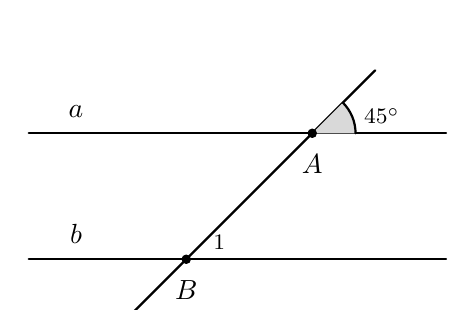
\begin{tikzpicture}[scale=1.0, line cap=round, line join=round]
    \coordinate (B) at (1.2, 0);
    \coordinate (A) at (2.8, 1.6);
    \draw[thick] (-0.8, 1.6) -- (4.5, 1.6);
    \node[above=2pt] at (-0.2, 1.6) {$a$};
    \draw[thick] (-0.8, 0) -- (4.5, 0);
    \node[above=2pt] at (-0.2, 0) {$b$};
    \draw[thick] ($(A)!1.5!(B)$) -- ($(B)!1.5!(A)$);
    \fill[gray!30] (A) -- ++(0:0.55) arc (0:45:0.55) -- cycle;
    \draw[thick] (A) ++(0:0.55) arc (0:45:0.55);
    \node[font=\footnotesize, right=1pt] at ($(A)+(0.5, 0.22)$) {$45^\circ$};
    \filldraw[black] (A) circle (1.5pt) node[below=4pt] {$A$};
    \filldraw[black] (B) circle (1.5pt) node[below=4pt] {$B$};
    \node[font=\footnotesize] at ($(B)+(0.42, 0.22)$) {$1$};
\end{tikzpicture}
}
\end{ex}

\begin{ex}
Điền cụm từ thích hợp vào chỗ trống: ''Qua một điểm nằm ngoài đường thẳng \dots đường thẳng song song với đường thẳng đó''.
\choice
{có vô số}
{\True chỉ có một}
{có hai}
{có ba}
\end{ex}


\vspace{1mm}
\noindent\textbf{BẢNG TRẢ LỜI TRẮC NGHIỆM PHẦN I:}
\begin{center}
\begin{tabular}{|c|c|c|c|c|c|c|c|c|c|c|c|c|}
\hline
\textbf{Câu} & \textbf{1} & \textbf{2} & \textbf{3} & \textbf{4} & \textbf{5} & \textbf{6} & \textbf{7} & \textbf{8} & \textbf{9} & \textbf{10} & \textbf{11} & \textbf{12} \\
\hline
\textbf{Chọn} & \rule{0pt}{0.65cm} & & & & & & & & & & & \\
\hline
\end{tabular}
\end{center}
\vspace{2mm}

\setcounter{ex}{0}
\noindent\textbf{\large PHẦN II. CÂU TRẮC NGHIỆM ĐÚNG SAI (2,0 điểm)}

\textit{Thí sinh trả lời câu 1 và câu 2. Trong mỗi ý a), b), c), d) ở mỗi câu, thí sinh chọn đúng hoặc sai.}

\vspace{1mm}
\begin{ex}
Cho biểu thức $A = \dfrac{3}{4} - \dfrac{1}{2} \cdot \left(-\dfrac{2}{3}\right)$ và $B = \left|-\dfrac{5}{6}\right|$. Xét tính đúng sai của các mệnh đề sau:
\choiceTF
{\True Giá trị của phép tính $\dfrac{1}{2} \cdot \left(-\dfrac{2}{3}\right)$ bằng $-\dfrac{1}{3}$}
{\True Giá trị của biểu thức $A$ bằng $\dfrac{13}{12}$}
{\True Giá trị của $B$ bằng $\dfrac{5}{6}$}
{Hiệu $A - B$ là một số hữu tỉ âm}
\end{ex}

\begin{ex}
Cho hai đường thẳng $xy$ và $zt$ song song với nhau. Đường thẳng $mn$ cắt $xy$ tại $M$ và cắt $zt$ tại $N$. Biết số đo góc $\widehat{xMN} = 55^\circ$. Xét tính đúng sai của các mệnh đề sau:
\choiceTF
{\True Góc $\widehat{MNt}$ và góc $\widehat{xMN}$ là hai góc so le trong}
{\True Số đo góc $\widehat{MNt}$ bằng $55^\circ$}
{\True Góc $\widehat{MNz}$ và góc $\widehat{xMN}$ là hai góc trong cùng phía}
{Số đo góc $\widehat{MNz}$ bằng $135^\circ$}
\end{ex}


\noindent\textbf{BẢNG TRẢ LỜI PHẦN II:}
\begin{center}
\begin{tabular}{|c|c|c|c|c||c|c|c|c|c|}
\hline
\textbf{Câu 1} & \textbf{a)} & \textbf{b)} & \textbf{c)} & \textbf{d)} & \textbf{Câu 2} & \textbf{a)} & \textbf{b)} & \textbf{c)} & \textbf{d)} \\
\hline
\textbf{Đ/S} & \rule{0pt}{0.6cm} & & & & \textbf{Đ/S} & & & & \\
\hline
\end{tabular}
\end{center}
\vspace{2mm}

\setcounter{ex}{0}
\noindent\textbf{\large PHẦN III. CÂU HỎI TRẢ LỜI NGẮN (1,0 điểm)}

\textit{Thí sinh trả lời câu 1 và câu 2. Điền kết quả vào ô trống.}

\vspace{1mm}
\begin{ex}
Tìm số hữu tỉ $x$, biết: $\left|x - \dfrac{1}{2}\right| = \dfrac{3}{2}$. \shortans{$x = 2$ hoặc $x = -1$}
\end{ex}

\begin{ex}
Cho hai đường thẳng song song $m$ và $n$. Đường thẳng $c$ cắt $m$ và $n$ lần lượt tại $A$ và $B$. Biết một góc so le trong $\widehat{A}_1 = 50^\circ$. Tính số đo góc đồng vị $\widehat{B}_1$ với góc $\widehat{A}_1$. \shortans{$50^\circ$}
\end{ex}


\newpage
\setcounter{ex}{0}
\noindent\textbf{\large PHẦN IV. TỰ LUẬN (4,0 điểm)}

\textit{Thí sinh trình bày chi tiết lời giải vào giấy làm bài.}

\vspace{1mm}
\begin{ex}
Thực hiện các phép tính sau (tính hợp lý nếu có thể):
\begin{enumerate}[label=\textbf{\alph*)}, leftmargin=0.8cm, itemsep=1pt]
\item $-\dfrac{3}{7} + \dfrac{5}{14} - \dfrac{1}{2}$;
\item $2{,}5 \cdot \left(-\dfrac{3}{5}\right) - 1{,}5 : \dfrac{5}{2}$;
\item $\left(-\dfrac{1}{3}\right)^2 - \dfrac{3}{8} \cdot \left(-\dfrac{2}{3}\right)^3 + \left|-2 \cdot \dfrac{1}{4}\right|$.
\end{enumerate}
\end{ex}
\vspace{1.5mm}

\begin{ex}

\begin{enumerate}[label=\textbf{\alph*)}, leftmargin=0.8cm, itemsep=1pt]
\item Sử dụng máy tính cầm tay làm tròn số $\sqrt{5}$ đến chữ số thập phân thứ nhất.
\item Tính độ dài cạnh hình vuông có diện tích bằng $36\text{ dm}^2$.
\end{enumerate}
\end{ex}
\vspace{1.5mm}

\begin{ex}
\immini{
Cho hình vẽ, biết $\widehat{mAB} = 60^\circ, \widehat{DBe} = 75^\circ, \widehat{ACD} = 60^\circ$.
\begin{enumerate}[label=\textbf{\alph*)}, leftmargin=0.8cm, itemsep=1pt]
\item Giải thích tại sao $AB \parallel CD$ và tính số đo $\widehat{CDt}$.
\item Vẽ $Ax$ là tia phân giác $\widehat{mAB}$, $Cy$ là tia phân giác $\widehat{ACD}$. Chứng minh $Ax \parallel Cy$.
\end{enumerate}
}{
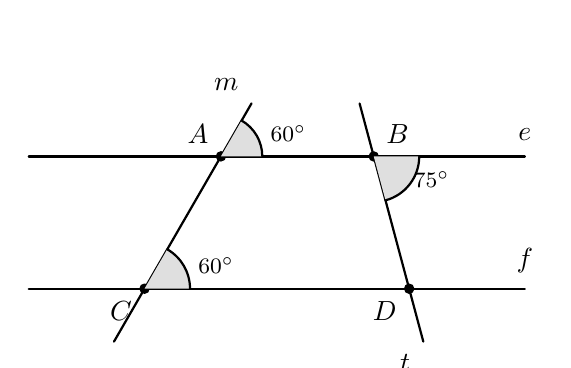
\begin{tikzpicture}[scale=1.05, line cap=round, line join=round]
    \draw[thick] (-0.8, 1.6) -- (5.2, 1.6) node[above=2pt] {$e$};
    \draw[thick] (-0.8, 0) -- (5.2, 0) node[above=2pt] {$f$};
    \coordinate (C) at (0.6, 0);
    \coordinate (A) at ($(C)+(60:1.848)$);
    \draw[thick] ($(C)!1.4!(A)$) node[above left=1pt] {$m$} -- ($(A)!1.4!(C)$);
    \coordinate (D) at (3.8, 0);
    \coordinate (B) at ($(D)+(105:1.656)$);
    \draw[thick] ($(D)!1.4!(B)$) -- ($(B)!1.4!(D)$) node[below left=1pt] {$t$};
    \filldraw[black] (A) circle (1.6pt) node[above left=1pt] {$A$};
    \filldraw[black] (C) circle (1.6pt) node[below left=1pt] {$C$};
    \filldraw[black] (B) circle (1.6pt) node[above right=1pt] {$B$};
    \filldraw[black] (D) circle (1.6pt) node[below left=1pt] {$D$};
    \fill[gray!25] (A) -- ++(0:0.5) arc (0:60:0.5) -- cycle;
    \draw[thick] (A) ++(0:0.5) arc (0:60:0.5);
    \node[font=\footnotesize, right=1pt] at ($(A)+(0.45, 0.28)$) {$60^\circ$};
    \fill[gray!25] (C) -- ++(0:0.55) arc (0:60:0.55) -- cycle;
    \draw[thick] (C) ++(0:0.55) arc (0:60:0.55);
    \node[font=\footnotesize, right=1pt] at ($(C)+(0.5, 0.28)$) {$60^\circ$};
    \fill[gray!25] (B) -- ++(0:0.55) arc (0:-75:0.55) -- cycle;
    \draw[thick] (B) ++(0:0.55) arc (0:-75:0.55);
    \node[font=\footnotesize, right=2pt] at ($(B)+(0.3, -0.28)$) {$75^\circ$};
\end{tikzpicture}
}
\end{ex}
\vspace{1.5mm}

\begin{ex}
Cho $M = \dfrac{1}{4} + \dfrac{1}{3^2} + \dfrac{1}{3^4} + \dfrac{1}{3^6} + \dots + \dfrac{1}{3^{802}}$. Chứng minh rằng $M < \dfrac{3}{8}$.
\end{ex}
\vspace{1.5mm}


\begin{center}
\rule{4cm}{0.4pt}\\
\textit{--- HẾT ---}
\end{center}
\end{document}
